\documentclass[mscthesis]{usiinfthesis}
\usepackage{lipsum}
\usepackage{color}
\usepackage{listings}
\usepackage{tikz}
\usetikzlibrary{calc}

% customizations
\lstset{
    linewidth=0.95\linewidth,
    breaklines=true,
    numbers=left,
    basicstyle=\small\ttfamily,
    numberstyle=\tiny,
    escapeinside={//*}{\^^M},
    mathescape=true
}
\DeclareMathOperator{\erf}{erf}
\lstdefinelanguage{algebra}
{morekeywords={import,sort,constructors,observers,transformers,axioms,if,
else,end},
sensitive=false,
morecomment=[l]{//s},
}

%===============================================================================
%%%%%%%%%%%%%%%%%%%%%%%%%%%%%%%%%%%%%%%%%%%%%%%%%%%%%%%%%%%%%%%%%%%%%%%%%%%%%%%%
\title{Accelerator for Event-based Failure Prediction} %compulsory
\specialization{Embedded Systems Design}%optional
\subtitle{Acceleration of an Extended Forward Algorithm for Failure Prediction
    on FPGA}
\author{Simon Maurer} %compulsory
\begin{committee}
    \advisor{Prof.}{Miroslaw}{Malek} %compulsory
    %\coadvisor{Prof.}{Student's}{Co-Advisor}{} %optional
\end{committee}
\Day{29.} %compulsory
\Month{Janaury} %compulsory
\Year{2014} %compulsory, put only the year
\place{Lugano} %compulsory

%\dedication{To my beloved} %optional
%\openepigraph{Someone said \dots}{Someone} %optional

%\makeindex %optional, also comment out \theindex at the end

\begin{document}

\maketitle %generates the titlepage, this is FIXED

\frontmatter %generates the frontmatter, this is FIXED

\begin{abstract}
\end{abstract}

%\begin{abstract}[Zusammenfassung]
%optional, use only if your external advisor requires it in his/er
%language 
%\\
%
%\lipsum
%\end{abstract}

\begin{acknowledgements}
\end{acknowledgements}

\tableofcontents 
\listoffigures %optional
\listoftables %optional

\mainmatter

%===============================================================================
%%%%%%%%%%%%%%%%%%%%%%%%%%%%%%%%%%%%%%%%%%%%%%%%%%%%%%%%%%%%%%%%%%%%%%%%%%%%%%%%
\chapter{Introduction}
\label{ch:intro}
In today's live it becomes increasingly important, that computer systems are
dependable. The reason being, that computer systems are used more and more in
areas where the failure of such a system can lead to catastrophic events.
Banking, public transportation and medical engineering are only a few examples
of areas employing large and extremely complex systems. The increasing
complexity of computer systems has a direct impact on their maintainability and
testability. It is simply impossible to guarantee that a piece of software comes
without any faults. On top of that, the same problematic arises with the
hardware components which also may contain faulty parts but also get
increasingly prone to failures due to decay of material.

In the event of a system failure it is of course desirable to fix the system as
soon as possible in order to minimize the downtime of the system (maximize the
availability). This can be accomplished by using different types of recovery
techniques, e.g. Check-pointing (create checkpoints to roll back/forward),
system replication (switch to a redundant system), fail over (reboot). All these
techniques require a certain amount of time to complete the recovery process,
time that is very expensive. In order to minimize this time, techniques have
been developed to anticipate upcoming failures. Such a technique is described in
\cite{salfner08}.

The work presents a new algorithm to predict failures and compares the results
with other techniques. The accuracy of the presented algorithm to predict
failures proves to be better compared to the other techniques, has however the
drawback of increased complexity and hence increased computation time. It is
very important to keep the computation overhead very low in order to maximize
the time between the prediction of a failure and the actual event of the
failure. One way to decrease the computation time is to design a hardware
accelerator for the prediction algorithm. The design of such an accelerator is
outlined in this document.

%-------------------------------------------------------------------------------
%===============================================================================
\section{Problem Statement}
\label{ch:_intro_prob}
%-------------------------------------------------------------------------------
%===============================================================================
\section{Motivation}
\label{ch:intro_mot}
The email of Felix left some doubts to whether the acceleration of the
algorithm is useful. The following list will give some arguments to justify
the work.
\begin{description}
    \item[Too many parameters to be identified, estimated and set] \hfill \\
        Considering an embedded system, this is usually not a problem because
        the parameters are defined during the design phase and will never be
        changed afterwards.
    \item[Limited performance scalability] \hfill \\
        There are studies available claiming otherwise. The discussion of
        Neumanns work will provide some arguments against this statement.
    \item[Industry trends point towards cloud] \hfill \\
        In embedded systems it will still be beneficial to predict failures of
        single nodes. It is however important to keep the power and
        computational footprint low. This will be one of the major challenges.
        On the other hand, I think it would also be possible to also use this
        algorithm to monitor a distributed system and predict failures. It is
        only a matter of getting defining the events to feed to the algorithm.
\end{description}

%-------------------------------------------------------------------------------
%===============================================================================
\section{Contributions}
\label{ch:intro_cont}
%-------------------------------------------------------------------------------
%===============================================================================
\section{Document Structure}
\label{ch:intro_struct}

%===============================================================================
%%%%%%%%%%%%%%%%%%%%%%%%%%%%%%%%%%%%%%%%%%%%%%%%%%%%%%%%%%%%%%%%%%%%%%%%%%%%%%%%
\chapter{State of the Art}
\label{ch:art}
This section provides an overview of the state of the art in the different
fields of research that are relevant for the thesis. This includes failure
prediction methods, existing solutions to accelerate failure prediction
algorithms and acceleration techniques in general.

%-------------------------------------------------------------------------------
%===============================================================================
\section{Failure Prediction}
\label{ch:art_pred}
A very detailed overview of failure prediction methods is given in
\cite{ACM10_Salfner}. The survey discusses i.a. the techniques used as
comparison in the main reference
\cite{lin88,IEEE90_lin,ICDM02_Vilalta,domeniconi02} as well as the technique
described in the main reference \cite{salfner08}.

More recent work uses hardware counters of a general purpose CPU and combines
them with software instrumentation to analyze failures of single processes (e.g
grep, flex, sed) \cite{FSE10_Yilmaz}. As industry heads more and more
towards cloud computing, it has been proposed to use information of interaction
between nodes (instead of analyzing single nodes) in order to analyze and
predict failures of a distributed system \cite{IEEE12_Salfner,DSN10_Oliner}.

%-------------------------------------------------------------------------------
%===============================================================================
\section{Accelerator}
\label{ch:art_acc}
The main goal of this master thesis is to accelerate an adaptation of the
forward algorithm. Proposals for a GPU based accelerator for the classic
forward algorithm are described in \cite{neumann11,liu09}. Further, several
proposals to accelerate the Viterbi algorithm (which is closely related to the
forward algorithm) have been published: \cite{ASAP12_Azhar} presents an
architecture for a lightweight Viterbi accelerator designed for an embedded
processor datapath, \cite{IPDPS07_Jacob,ICS06_Maddimsetty,IPDPS07_Oliver}
describe a FPGA based accelerator for protein sequence HHM search and
\cite{IPDPS09_Walters} describes i.a. an approach to accelerate the Viterbi
algorithm from the HMMER library using GPUs.

Focusing on a more general approach for acceleration, \cite{ARITH13_Kadric}
proposes an FPGA implementation of a parallel floating point accumulation and
\cite{ITNG07_Yang} describes the implementation of a vector processor on
FPGA.

Quite some research has been done on the question what type of technology
should be used to accelerate certain algorithms: \cite{SASP08_Che} presents
a performance study of different applications accelerated on a multicore CPU,
on a GPU and on a FPGA, \cite{FPL10_Jones} discusses the suitability of FPGA
and GPU acceleration for high productivity computing systems (HPCS) without
focusing on a specific application and \cite{ISVLSI10_Kestur} also focuses on
HPCS but uses the Basic Linear Algebra Subroutines (BLAS) as comparison and
also takes CPUs into account.

It may be interesting to also think about an acceleration of the model
training. Similar work has been done by accelerating SVMs (Support Vector Machines):
\cite{FCCM09_Cadambi} describes a FPGA based accelerator for the SVM-SMO
(support vector machine - sequential minimal optimization) algorithm used in
the domain of machine learning and \cite{IEEE03_Anguita} proposes a new algorithm
and its implementation on a FPGA for SVMs.

%===============================================================================
%%%%%%%%%%%%%%%%%%%%%%%%%%%%%%%%%%%%%%%%%%%%%%%%%%%%%%%%%%%%%%%%%%%%%%%%%%%%%%%%
\chapter{Event-based Failure Prediction}
\label{ch:event}

This section provides a brief overview of the computational steps done by the
proposed algorithm \cite{salfner08}.

\emph{\color{red}brief description of the idea behind the algorithm, HSMM, Events, etc}

To be able to understand the formal expression of the algorithm, first
a definition of the used parameters is provided.
\begin{itemize}
    \item N: number of states
    \item M: number of observation symbols
    \item L: observation sequence length
    \item R: number of cumulative probability distributions (kernels)
\end{itemize}
The delay of the event at time $ t_k $ with respect to the event at time
$ t_{k-1} $ is described as
\begin{equation}
    d_k = t_k-t_{k-1}
\end{equation}

%-------------------------------------------------------------------------------
%===============================================================================
\section{Data Processing}
\label{ch:event_data}

%-------------------------------------------------------------------------------
%===============================================================================
\section{Model Training}
\label{ch:event_train}

One part of the algorithm is the model training. This part is not described
here. The features to be trained by the model training are however important
in this context because they are used by the adapted forward algorithm.
Following the features:
\begin{itemize}
    \item $ \pi_i $, forming the initial state probability vector
        $ \boldsymbol{\pi} $ of size $ N $
    \item $ b_i(o_j) $, forming the emission probability matrix $ B $ of size
        $ N \times M $
    \item $ p_{ij} $, forming the matrix of limiting transmission probabilities
        $ P $ of size $ N \times N $
    \item $ \omega_{ij, r} $, the weights of the kernel $ r $
    \item $ \theta_{ij, r} $, the parameters of the kernel $ r $
\end{itemize}

%-------------------------------------------------------------------------------
%===============================================================================
\section{Sequence Processing}
\label{ch:event_sequ}

The following description will provide a complete blueprint of the adapted
forward algorithm, that allows to implement it, but without any explanations or
proofs related to the formulation. The adapted forward algorithm is defined as
follows:
\begin{equation}
    \label{eq:forward_init}
    \alpha_0(i) = \pi_{i}b_{s_i}(O_0) \\
\end{equation}
\begin{equation}
    \label{eq:forward}
    \alpha_k(j) = \sum_{i=1}^{N} \alpha_{k-1}(i) v_{ij}(d_k) b_{s_j}(O_k);
    \quad 1 \leq k \leq L
\end{equation}
where
\begin{equation}
    \label{eq:V}
    v_{ij}(d_k) = \left\{
        \begin{array}{l l}
            p_{ij} d_{ij}(d_k)
                & \quad \text{if $j \neq i$}\\
            1 - \sum\limits_{\substack{h=1 \\ h \neq i}}^{N} p_{ih} d_{ih}(d_k)
                & \quad \text{if $j = i$}
        \end{array} \right.
\end{equation}
with
\begin{equation}
    \label{eq:D}
    d_{ij}(d_k) = \sum_{r=1}^{R} \omega_{ij,r}\kappa_{ij,r}(d_k|\theta_{ij, r})
\end{equation}
forming the matrix of cumulative transition duration distribution functions
$ D(d_k) $ of size $ N \times N \times L $.

For simplification reasons, only one kernel is used. Due to this, the kernel
weights can be ignored. Equation \ref{eq:D} can then be simplified:
\begin{equation}
    \label{eq:D_fact}
    d_{ij}(d_k) = \kappa_{ij}(d_k | \theta_{ij})
\end{equation}
Choosing the Gaussian cumulative distribution results in the kernel parameters
$ \mu_{ij} $ and $ \sigma_{ij} $:
\begin{equation}
    \label{eq:kernel}
    \kappa_{ij, gauss}(d_k | \mu_{ij}, \sigma_{ij}) = 
    \frac{1}{2}\bigg [1 + \erf \big (\frac{d_k - \mu_{ij}}{\sqrt 2 \sigma_{ij}}\big )
        \bigg ]
\end{equation}

The last set of forward variables $ \alpha_L $ are then summed up to compute
a probabilistic measure for the similarity of the observed sequence compared to
the sequences in the training data set. This is called the sequence likelihood:
\begin{equation}
    \label{eq:P}
    P(\boldsymbol{o}|\lambda) = \sum\limits_{i=1}^{N} \alpha_L(i)
\end{equation}
where $ \lambda = \{\boldsymbol{\pi}, P, B, D(d_k) \} $.

To prevent $ \alpha $ from going to zero very fast, at each step of the forward
algorithm a scaling is performed:
\begin{equation}
    \alpha_k(i) = c_k \alpha_k(i)
\end{equation}
with
\begin{equation}
    c_k = \frac{1}{\sum\limits_{i=1}^{N} \alpha_k(i)}
\end{equation}

By applying scaling, instead of the sequence likelihood (equation \ref{eq:P}),
the sequence log-likelihood must be computed:
\begin{equation}
    \label{eq:Plog}
    \log(P(\boldsymbol{o}|\lambda)) = -\sum\limits_{k=1}^{L} \log c_k
\end{equation}
where $ \lambda = \{\boldsymbol{\pi}, P, B, D(d_k) \} $.

%-------------------------------------------------------------------------------
%===============================================================================
\section{Classification}
\label{ch:event_class}

\emph{\color{red}explain classification}

and finally the
classification is performed:
\begin{equation}
    \label{eq:class}
    \text{class}(s) = F \iff \max_{i=1}^{u} \big [
        \log P(\boldsymbol{s}|\lambda_i)
    \big ] - \log P(\boldsymbol{s}|\lambda_0) > \log \theta
\end{equation}
with
\begin{equation}
    \label{eq:class_thresh}
    \theta = \frac{(r_{\bar{F}F} - r_{\bar{F}\bar{F}})P(c_{\bar{F}})}
        {(r_{F \bar{F}} - r_{FF})P(c_{F})}
\end{equation}
To calculate $ \theta $, the following parameters need to be set:
\begin{itemize}
    \item $ P(c_{\bar{F}}) $: prior of non-failure class
    \item $ P(c_F) $: prior of failure class
    \item $ r_{\bar{F}\bar{F}} $: true negative prediction
    \item $ r_{FF} $: true positive prediction
    \item $ r_{\bar{F}F} $: false positive prediction
    \item $ r_{F\bar{F}} $: false negative prediction
\end{itemize}

%===============================================================================
%%%%%%%%%%%%%%%%%%%%%%%%%%%%%%%%%%%%%%%%%%%%%%%%%%%%%%%%%%%%%%%%%%%%%%%%%%%%%%%%
\chapter{Acceleration}
\label{ch:acc}

Challenges of the acceleration
\begin{itemize}
    \item implementation of exp and log function (LUT, Taylor, ...)
    \item floating points vs fixed points
    \item precision
    \item choice of accelerator (Type, Model)
    \item find available options for parallelization
\end{itemize}

Ideas on how to accelerate the online part of the algorithm
\begin{itemize}
    \item use high speed multiplier-accumulator (MAC) devices on a FPGA
    \item use MACs only on integer numbers and compute FP later manually
    \item precompute known factors and store them in order to simplify online
        computation (e.g. parts of the kernel, classification threshold, ...).
    \item \dots
\end{itemize}

Possible optimizations of the algorithm:
\begin{itemize}
    \item use a regularization term in the cost function to prevent overfitting
    \item incorporate the offline part of the algorithm into the online part in
        order to deal with model aging
    \item \dots
\end{itemize}

%-------------------------------------------------------------------------------
%===============================================================================
\section{Theoretical Analysis}
\label{ch:acc_theo}

%-------------------------------------------------------------------------------
\subsection{Serial Implementation}

Script to run a sliding window over the sequence
\lstinputlisting[language=Octave]{../accelerator/model/main_script.m}
Forward Algorithm
\lstinputlisting[language=Octave]{../accelerator/model/forward_s.m}
Initialisation of each step
\lstinputlisting[language=Octave]{../accelerator/model/forward_s_init.m}
Computation per Observation Symbol
\lstinputlisting[language=Octave]{../accelerator/model/forward_s_step.m}
Extension of Forward Algorithm
\lstinputlisting[language=Octave]{../accelerator/model/compute_tp.m}

%-------------------------------------------------------------------------------
\subsection{Available Parallelism}

\begin{itemize}
    \item pipelining
    \item replication of independent blocks
\end{itemize}

%-------------------------------------------------------------------------------
\subsection{Scaling and Data Representation}

Scaling may be applied to prevent that the continuous multiplication of numbers
smaller than one (e.g. probabilities) result in zero because of the limited
accuracy by digitally representing fractional numbers. Scaling does not
influence the order of complexity of the algorithm. By introducing scaling, the
complexity of calculating one $ \alpha_k $ vector goes from $ N^2 $ (no
scaling) to $ N^2 + 2N + 1 $ (scaling), which is the same order $ O(N^2) $.
However, the introduction of scaling may increase the usage of recourses
significantly: In order to scale $ \alpha_k $, the division operation is used
to compute the scaling factor.  Division is far more complex than
multiplication and hence uses more recourses.  Additionally, instead of the
sequence likelihood (equation \ref{eq:P}) the sequence log-likelihood (equation
\ref{eq:Plog}) needs to be computed, with the even more complex log operation.

In order to limit the amount of necessary division operations, it is beneficial
to consider the following: Rather than scaling each element of $ \alpha_k $ by
dividing it by a scaling factor ($ N $ divisions), first the inverse of the
scaling factor can be computed, which is then multiplied with each element of
$ \alpha_k $ (one division and $ N $ multiplications). 

To compute the log-likelihood, $ N $ log and $ N $ sum operations are
necessary, in comparison to $ N $ sum operations for the likelihood. In terms
of memory, the log-likelihood is more complex because the scaling coefficients
of each $ \alpha_k $ are used and need to be stored, while for the likelihood
only the last set of forward variables $ \alpha_L $ are used.

Another aspect to consider is the choice of data representation (floating point
vs. fixed point). This depends on one hand on the necessary precision and on
the other hand on the choice of accelerator type.  While general purpose
hardware such as CPU, GPU and DSP (to some degree) offer an abstraction to make
the representation type transparent to the developer, specialized hardware such
as FPGA or ASCI offer no such abstraction. For the later devices, floating
point operations increase the complexity of the hardware design and the
necessary hardware resources considerably. In terms of performance, general
purpose devices benefit also from a sparse usage of floating point values. The
complexity of the software development however is only marginally or not
affected at all by the choice of data representation.

If by choice, scaling is omitted, a fixed point representation will not be
possible, due to the rapid convergence towards zero by continuously multiplying
probabilities together. This implies, that by omitting scaling to save
resources, a floating point representation must be used, which again increases
the resource requirements or has a negative impact on performance (or both).

The trade-off between the choice of using scaling or not versus the choice of
the precision and the data representation, will be analyzed in more detail in
chapter \ref{ch:acc_des}, when the technology of the accelerator has been
chosen.

Scaling in general:
\begin{equation}
    \sum\limits_{i=1}^{N} \pi_i = 1
\end{equation}
\begin{equation}
    \sum\limits_{j=1}^{N} v_{ij}(d_k) = 1
\end{equation}
\begin{equation}
    \sum\limits_{j=1}^{M} b_{ij} = 1
\end{equation}
on average each\\
$ \alpha_1 = \frac{1}{NM} $\\
$ \alpha_2 = N\frac{1}{NM}\frac{1}{NM} = \frac{1}{NM^2} $\\
$ \alpha_3 = N\frac{1}{NM}\frac{1}{NM^2} = \frac{1}{NM^3} $\\
\dots\\
$ \alpha_L = \frac{1}{NM^L} $\\
assuming no precision loss at each computational step $ k $, on average a
scaling factor of $ \frac{1}{M} $ is necessary in each step $ k $.

%-------------------------------------------------------------------------------
\subsection{Computation of Extension}
This computation is very expensive but needs only to be computed once per dk.
(Unlike the alphas, which need to be recomputed for the same dk because they
depend on the previous alpha).

Maybe use a very specialized unit (ASIC) just for the computation of the
cumulative distribution function.

%-------------------------------------------------------------------------------
%===============================================================================
\section{Choice of Accelerator Type}
\label{ch:acc_choice}

%-------------------------------------------------------------------------------
\subsection{CPU}
\begin{itemize}
    \item pro
    \begin{itemize}
        \item fast and easy implementation (availability of /, exp, log,
            floating points)
        \item high precision (double, long double)
        \item high frequency (up to 3 GHz)
    \end{itemize}
    \item contra
    \begin{itemize}
        \item high power consumption
        \item limited parallelization (limited number of cores)
        \item large overhead (because of instruction pipeline)
        \item fixed architecture (memory, computation units)
    \end{itemize}
\end{itemize}

%-------------------------------------------------------------------------------
\subsection{GPU}
\begin{itemize}
    \item pro
    \begin{itemize}
        \item SIMD: a lot of streaming processors for a low price
        \item a lot of fast onboard memory
        \item high frequency
        \item high precision
        \item simple implementation (availability of /, exp, log,
            floating points)
    \end{itemize}
    \item contra
    \begin{itemize}
        \item high power consumption
        \item overhead for simple instructions (instruction pipeline)
        \item fixed architecture (memory, computation units)
    \end{itemize}
\end{itemize}

%-------------------------------------------------------------------------------
\subsection{FPGA}
\begin{itemize}
    \item pro
    \begin{itemize}
        \item low power consumption
        \item low overhead
        \item flexibility
        \item optimized floating point representation (small values)
    \end{itemize}
    \item contra
    \begin{itemize}
        \item low frequency
        \item parallelization is expensive
        \item precision is expensive
        \item complex implementation
    \end{itemize}
\end{itemize}

%-------------------------------------------------------------------------------
\subsection{ASIC}
\begin{itemize}
    \item pro
    \begin{itemize}
        \item very low power consumption
        \item no overhead
        \item very flexible
        \item optimized floating point representation (small values)
    \end{itemize}
    \item contra
    \begin{itemize}
        \item very expensive
        \item very complex implementation
    \end{itemize}
\end{itemize}

%-------------------------------------------------------------------------------
\subsection{Conclusion}
\begin{itemize}
    \item target is an embedded system (low power)
    \item optimize memory hierarchy
    \item student budget
    \item -> use FPGA
    \item only standard forward algorithm
    \item do not use scaling because of division. Instead use custom FP
        representation
\end{itemize}

basic implementation without extension and scaling
\lstinputlisting[language=Octave]{../accelerator/model/forward_s_basic.m}

%-------------------------------------------------------------------------------
%===============================================================================
\section{Design and Implementation}
\label{ch:acc_des}
\begin{itemize}
    \item parallelization of one of nested for-loop or pipeline the loops
    \item fully pipelined MACC
\end{itemize}

To design the accelerator, the top-down approach was applied: the algorithm is
broken down into blocks, where each of them is broken down further until the
basic functional blocs of the FPGA can be used for the implementation. The
implementation follows then the bottom-up approach where each sub-block is
implemented and tested. Completed blocks are grouped together to bigger blocks
until finally there is only one big block remaining, describing the complete
algorithm.

%-------------------------------------------------------------------------------
\subsection{Precision}

Modern FPGAs contain hardware blocks (DSP slices) that are heavily optimized
for multiply-accumulate operations as they are often used for DSP applications.
These devices only operate on integer values. However, the forward algorithm
requires to multiply and accumulate probabilities, i.e. fractional numbers. To
being able to use the DSP slices of the FPGA, some hardware must be built
around such a slice in order to get a hardware block that can handle the
multiplication and accumulation of probabilities. To do this, the choice of
data representation must be made (floating point vs fixed point). First the
assumption that all operations must be done with floating point numbers is
discussed.

\emph{\color{red}the following points need to be explained in more detail}

Floating Point Facts:
In order to multiply two floating point numbers, the mantissas of
both numbers are multiplied and the exponents are added (the sign can be
ignored, as probabilities are always positive). For the multiplication of the
mantissas the DSP slices can be used. In parallel to this operation, an
external adder can add up the exponents. Now the tricky part: to being able to
add floating point numbers the exponents of the numbers must be equal. To
achieve that, the difference of the two exponents is calculated and then the
mantissa of the number with the lower exponent must be shifted by this
difference (and possibly rounded/truncated). This process is called
normalizing. Then the mantissas can be added. Finally the resulting value
needs to be normalized again.

Scaling: By using floating points, scaling becomes superfluous because the
exponent allows to represent very small numbers (not respecting IEEE
representations).

Truncation: after the multiply accumulate operation the resulting mantissa of
48 bits must be truncated to 25 bits. To achieve better results, a rounding
operation can be applied.

Fixed Point Facts:
before each multiplication, the operands need to be reduced from 48 to 18 resp
25 bits. This must be done by either truncating/rounding the final value or by
scaling or by doing both.

Scaling: The proposed scaling method is not usable in this implementation
because of the division operation. Instead, a scaling in base of 2 should be
used (shift): In every clock cycle a new value is added to the previous one.
The masked result can be compared to a bit stream of zeros. A match directly
gives the amount of leading zeros (using the number of times the mask has been
shifted). If there is no match, shift the mask and compare in the next cycle.
This operation is done with every alpha, while the lowest value of leading
zeros is kept. Using this method, in most cases at the end of adding up all the
values, the least number of leading zeros of the N alphas will be known. If in
the worst case after the addition of the last alpha-component there is
a non-match, the pipeline must be stalled and the right leading zeros number
must be found by shifting the mask further to the left. To do the masked
comparison, the pattern comparing unit of the DSP-slice of the FPGA can be
used. The stored values $ \pi $, $ B $ and $ TP $ can be preprocessed and
scaled, in order to reduce the number of minimal leading zeros to zero. These
scaling factors will then be used to recompute the real sequence likelihood.

Truncation: a simple solution is to chop off the leading zeros (as counted) and
truncate the value by only using the following 25 bits after the last leading
zero. A more precise method would be to use rounding.

%-------------------------------------------------------------------------------
\subsection{Data Storage Management}

\emph{\color{red}the following points need to be explained in more detail}

Facts:
in each kth step $ N^2*TP $ values and $ N*B $ values are necessary. In case of
the parallel version, each clock cycle $ N*TP $ and one B value must be made
available. In case of the serial version one TP or B vale must be made
available. By reading directly from the RAM, 16 bits can be read with a bus
frequency of 104MHz. Running the pipeline at 52MHz, the necessary data can be
provided at each clock cycle in case of the serial implementation. If the
parallel implementation should be used, an internal memory must be built.

\begin{itemize}
    \item real-time (time constraints on every Ps) vs on-line (use buffer to
        optimize throughput)
    \item memory hierarchy: at startup copy from flash to ram, then use pipeline
        to preload values from ram into registers.
\end{itemize}

%-------------------------------------------------------------------------------
\subsection{Top View}
\emph{\color{red}better title?}

The computation of the likelihood is divided in $ L $ steps: the
initialization, $ L-2 $ identical intermediate steps and the finalization.
$ N $ initial forward variables $ \alpha_0 $. Each intermediate step computes
$ N $ intermediate forward variables $ \alpha_k $ and the final step calculates
the last set of $ N $ forward variables $ \alpha_L $ as well as the likelihood.
Each step takes the emission probabilities $ b_i(o_k) $ corresponding to the
observation symbol $ o_k $ and constant factors as input. Because of the
recursive nature of the algorithm, all steps (except the initialization) depend
on the previously computed forward variables. For this reason a direct
parallelization of the steps is not possible. However, at every arrival of
a new observation symbol, the last $ L $ elements of the observation symbol
sequence are used to compute the likelihood. Hence, it is very beneficial to
pipeline the steps. To do this, each step corresponds to a pipeline stage and is
realized in hardware and connected as represented in the figure \ref{fig:arch}.
With this configuration, a likelihood is computed at every completion of a step
with a latency of $ L * t_{step_{max}} $, where $ t_{step_{max}} $ is the time
needed to complete the computation of the most complex step (each stage of the
pipeline must take the same amount of clock cycles). Additionally the
configuration allows to load the constants $ TP $ and the emission
probabilities $ b_i(o_k) $ for all steps at the same time, which reduces the
load operations considerably. In the following sections, each dissimilar block
is described in more detail.

%\emph{\color{red}example on how the pipeline works}
%at time $ t $ a new observation symbol $ o_t $ arrives and the corresponding
%emission probabilities $ B(o_t) $ are entered as input into all the stages of
%the pipeline. At time $ t+1 $ all the pipeline steps have completed their
%computation, enter their result as input into the next pipeline stage and
%receive new emission probabilities $ B(o_{t+1}) $

\emph{\color{red}add step k to the figure \ref{fig:arch}}

\begin{figure}[h]
    \newcommand*{\Width}{3.0}
\newcommand*{\Height}{2.0}
\tikzstyle{block} = [draw, minimum width=\Width cm, minimum height=\Height cm, anchor=south west, text width=2cm, align=center]
\begin{tikzpicture}[>=stealth]
%coordinates
\coordinate (orig)   at (0,0);
\coordinate (nSi)    at (2,7.5);
\coordinate (nS1)    at (2,4.5);
\coordinate (nSL)    at (2,1);
\coordinate (pSi1)   at (5.5,8.5);
\coordinate (pSi2)   at (5.5,7);
\coordinate (pSi3)   at (1.5,7);
\coordinate (pSi4)   at (1.5,6);
\coordinate (pS11)   at (5.5,5.5);
\coordinate (pS12)   at (5.5,4);
\coordinate (pS13)   at (1.5,4);
\coordinate (pS14)   at (1.5,3.5);
\coordinate (pS15)   at (1.5,3);
\coordinate (pS16)   at (1.5,2.5);
\coordinate (pPI)    at (0,9);
\coordinate (pB)     at (0,8.5);
\coordinate (pBi)    at (1,8.5);
\coordinate (pB1)    at (1,5.5);
\coordinate (pBL1)   at (1,3.5);
\coordinate (pBL2)   at (1,3);
\coordinate (pBL)    at (1,2);
\coordinate (pTP)    at (0,5);
\coordinate (pTP1)   at (0.5,5);
\coordinate (pTPL1)  at (0.5,3.5);
\coordinate (pTPL2)  at (0.5,3);
\coordinate (pTPL)   at (0.5,1.5);
\coordinate (pP)     at (6,2);

%nodes
\node[block] (Si) at (nSi) {Step 1\\(Init)};
\node[block] (S1) at (nS1) {Step 2};
\node[block] (SL) at (nSL) {Step L};

\node (nPI) at (pPI) {$ \pi $};
\node (nB) at (pB) {$ B(o_k) $};
\node (nTP) at (pTP) {$ TP $};
\node (nP) at (pP) {$ P $};

\path[fill] (pBi) circle[radius=1pt] (pB1) circle[radius=1pt];
\path[fill] (pTP1) circle[radius=1pt];

\draw[->] (nPI) -- ($(nSi) + (0,1.5)$);
\draw[->] (nB) -- ($(nSi) + (0,1)$);
\draw[->] (pBi) -- (pB1) -- ($(nS1) + (0,1)$);
\draw (pB1) -- (pBL1);
\draw[dotted] (pBL1) -- (pBL2);
\draw[->] (pBL2) -- (pBL) -- ($(nSL) + (0,1)$);
\draw[->] (nTP) -- ($(nS1) + (0,0.5)$);
\draw (pTP1) -- (pTPL1);
\draw[dotted] (pTPL1) -- (pTPL2);
\draw[->] (pTPL2) -- (pTPL) -- ($(nSL) + (0,0.5)$);

\draw[->] ($(nSi) + (\Width,1)$) -- (pSi1) -- (pSi2) -- (pSi3) -- (pSi4) -- ($(nS1) + (0,1.5)$);
\draw ($(nS1) + (\Width,1)$) -- (pS11) -- (pS12) -- (pS13) -- (pS14);
\draw[dotted] (pS14) -- (pS15);
\draw[->] (pS15) -- (pS16) -- ($(nSL) + (0,1.5)$);
\draw[->] ($(nSL) + (\Width,1)$) -- (nP);

\end{tikzpicture}

    \centering
    \def\svgwidth{\columnwidth}
    \caption{Top View of the Architecture}
    \label{fig:arch}
\end{figure}

%-------------------------------------------------------------------------------
\subsection{Initialization}

Figure \ref{fig:init_s} shows the necessary operation to compute every i-th
component of the first forward variable $ \alpha_1 $ in the initialization
step.  The $ N $ components of $ \alpha_1 $ can be computed one by one when
only one such structure is implemented in hardware. Assuming a fully
pipelineable multiplier, one component of $ \alpha_1 $ appears in the output
register at every cycle (with a latency of $ S $ cycles, where $ S $ is the
number of pipeline stages in the multiplier). To compute all $ N $ components
of $ \alpha_1 $ with this structure, $ N + S $ cycles are necessary.
Alternatively the complete initialization can be fully parallelized if the
structure \ref{fig:init_s} is replicated $ N $ times. In this case, all
$ N $ components of $ \alpha_1 $ appear at the same time, after $ S $ cycles in
the output registers. If such a heavy parallelization is useful will be
analyzed after all stages have been described.

%\emph{\color{red}add input registers to figure \ref{fig:init}}

%\begin{figure}[h]
%    \newcommand*{\Width}{2.5}
\newcommand*{\Height}{1.5}
\tikzstyle{block} = [draw, minimum width=\Width cm, minimum height=\Height cm, anchor=south west, text width=2cm, align=center]
\begin{tikzpicture}[>=stealth]
%coordinates
\coordinate (orig)   at (0,0);
\coordinate (nMul)   at (1,1);
\coordinate (nReg)   at (5,1);
\coordinate (pPI)    at (0,2);
\coordinate (pB)     at (0,1.5);
\coordinate (pA)     at (8.5,1.75);

%nodes
\node[block] (Mul) at (nMul) {Mul};
\node[block] (Reg) at (nReg) {Reg};

\node (nPI) at (pPI) {$ \pi_i $};
\node (nB) at (pB) {$ b_i(o_k) $};
\node (nA) at (pA) {$ \alpha_i $};

\draw[->] (nPI) -- ($(nMul) + (0,1)$);
\draw[->] (nB) -- ($(nMul) + (0,0.5)$);
\draw[->] ($(nMul) + (\Width,0.75)$) -- ($(nReg) + (0,0.75)$);
\draw[->] ($(nReg) + (\Width,0.75)$) -- (nA);

\end{tikzpicture}

%    \centering
%    \def\svgwidth{\columnwidth}
%    \caption{Initialization step}
%    \label{fig:init}
%\end{figure}
\begin{figure}[h]
    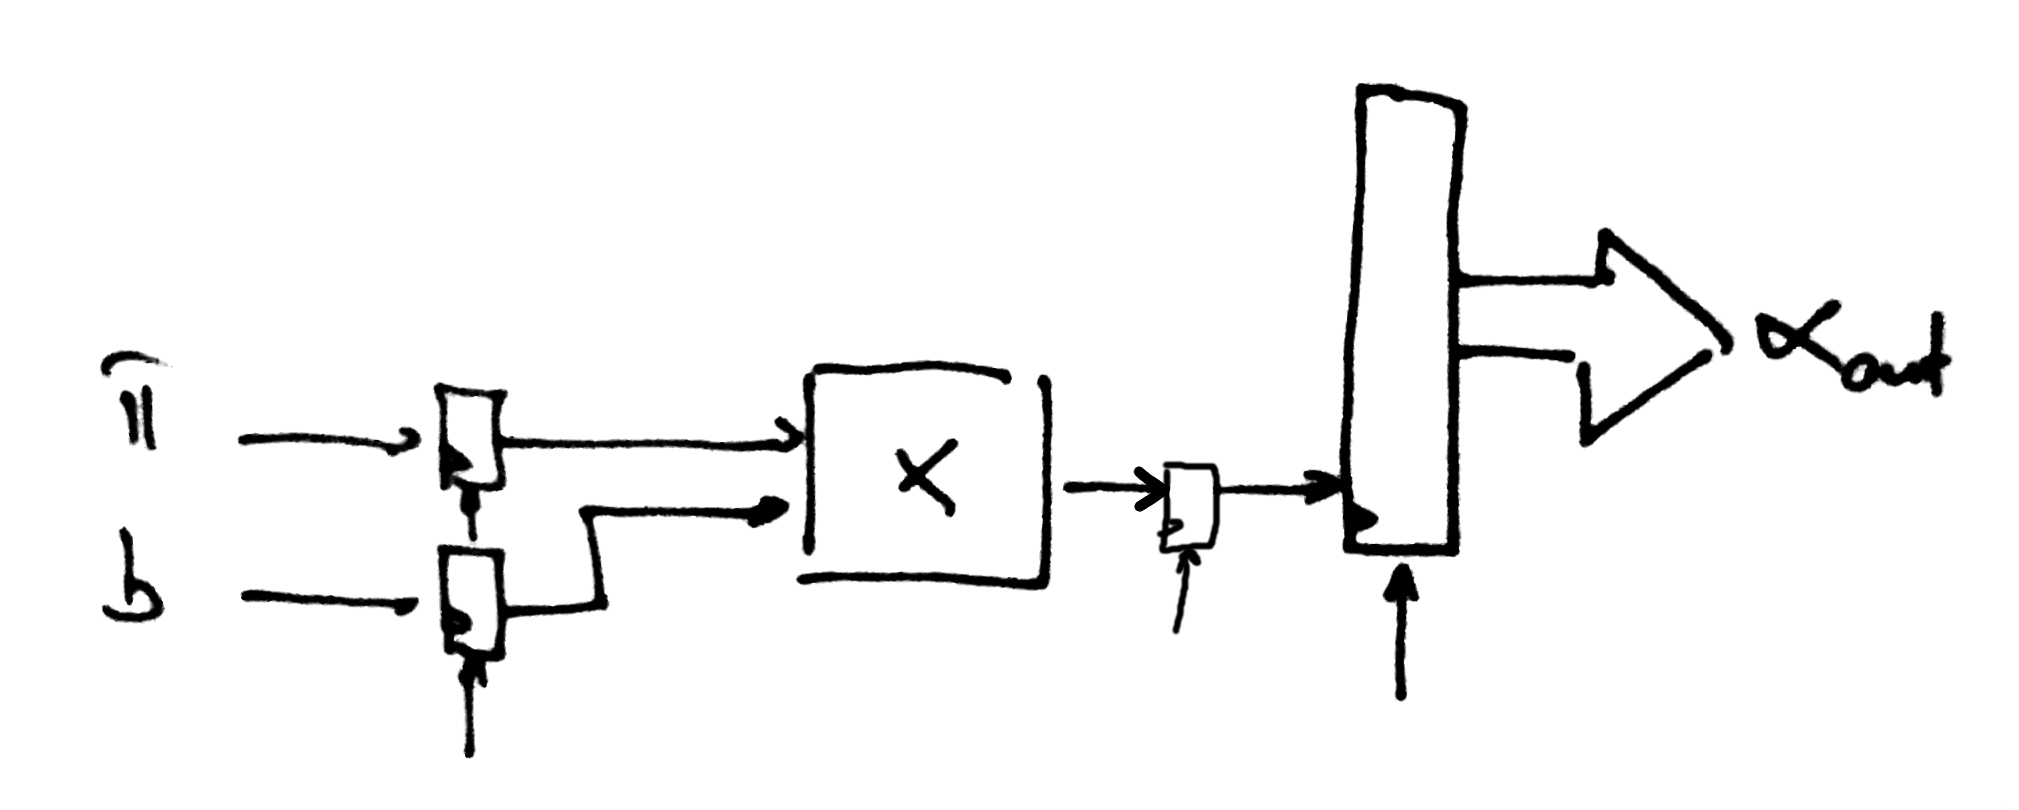
\includegraphics[width=1\columnwidth]{arch_init_s.png}
    \caption{Initialisation step with one MACC}
    \label{fig:init_s}
\end{figure}

%-------------------------------------------------------------------------------
\subsection{k-th Forward Variable}
\emph{\color{red}better title?}

\begin{itemize}
    \item one pipelined MACC for the computation of all elements
    \item $ N $ pipelined MACC, each computing one $ \alpha_k $
    \item use optimized Matrix-Vector-Vector multiplication
        $ \alpha_{k+1} = TP * \alpha_k * B(o_k) $
        \cite{FCCM12_Kestur, ITNG07_Yang}
\end{itemize}

\begin{figure}[h]
    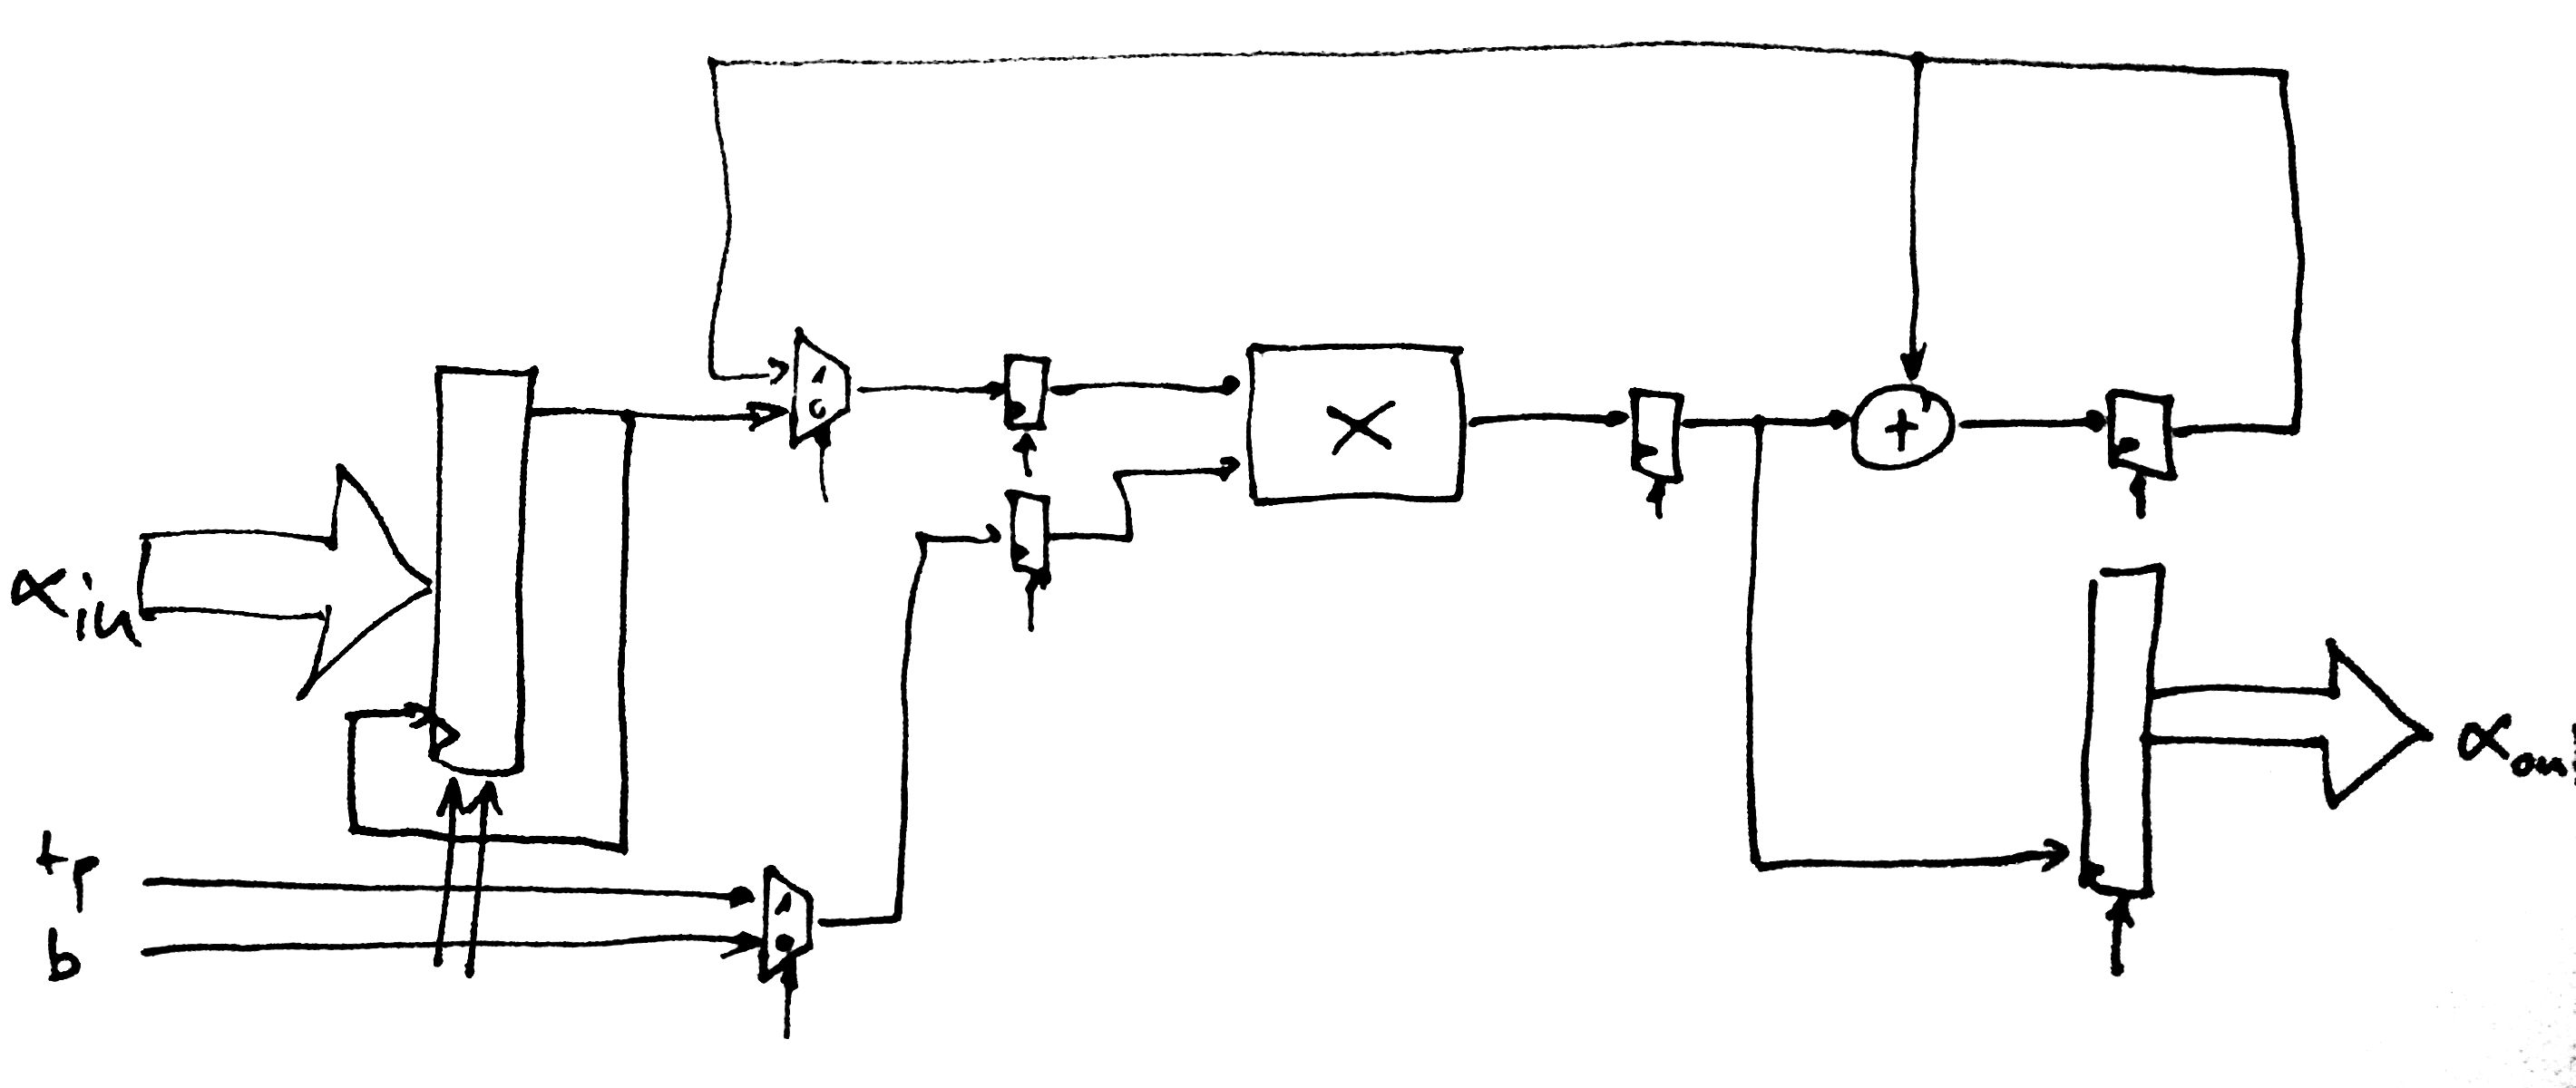
\includegraphics[width=1\columnwidth]{arch_step_s.png}
    \caption{k-th step with one MACC unit}
    \label{fig:step_s}
\end{figure}
\begin{figure}[h]
    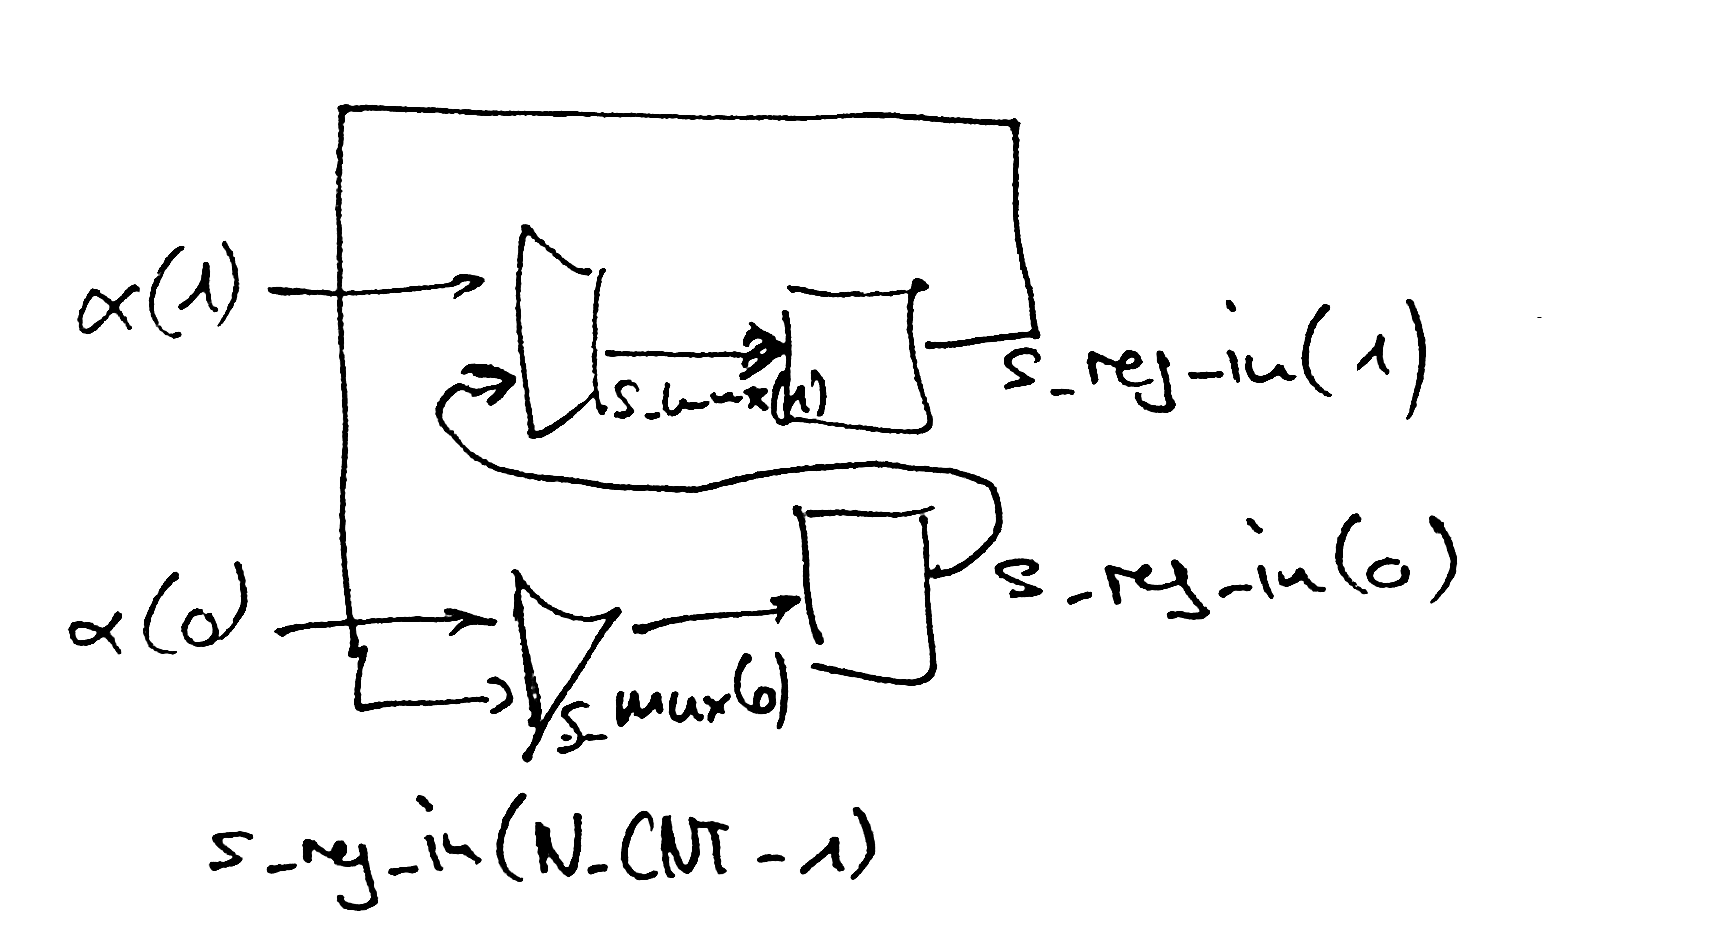
\includegraphics[width=1\columnwidth]{./arch_shift_reg_s.png}
    \caption{Example of input shift register with N=2}
    \label{fig:shift_reg_s}
\end{figure}

\begin{figure}[h]
    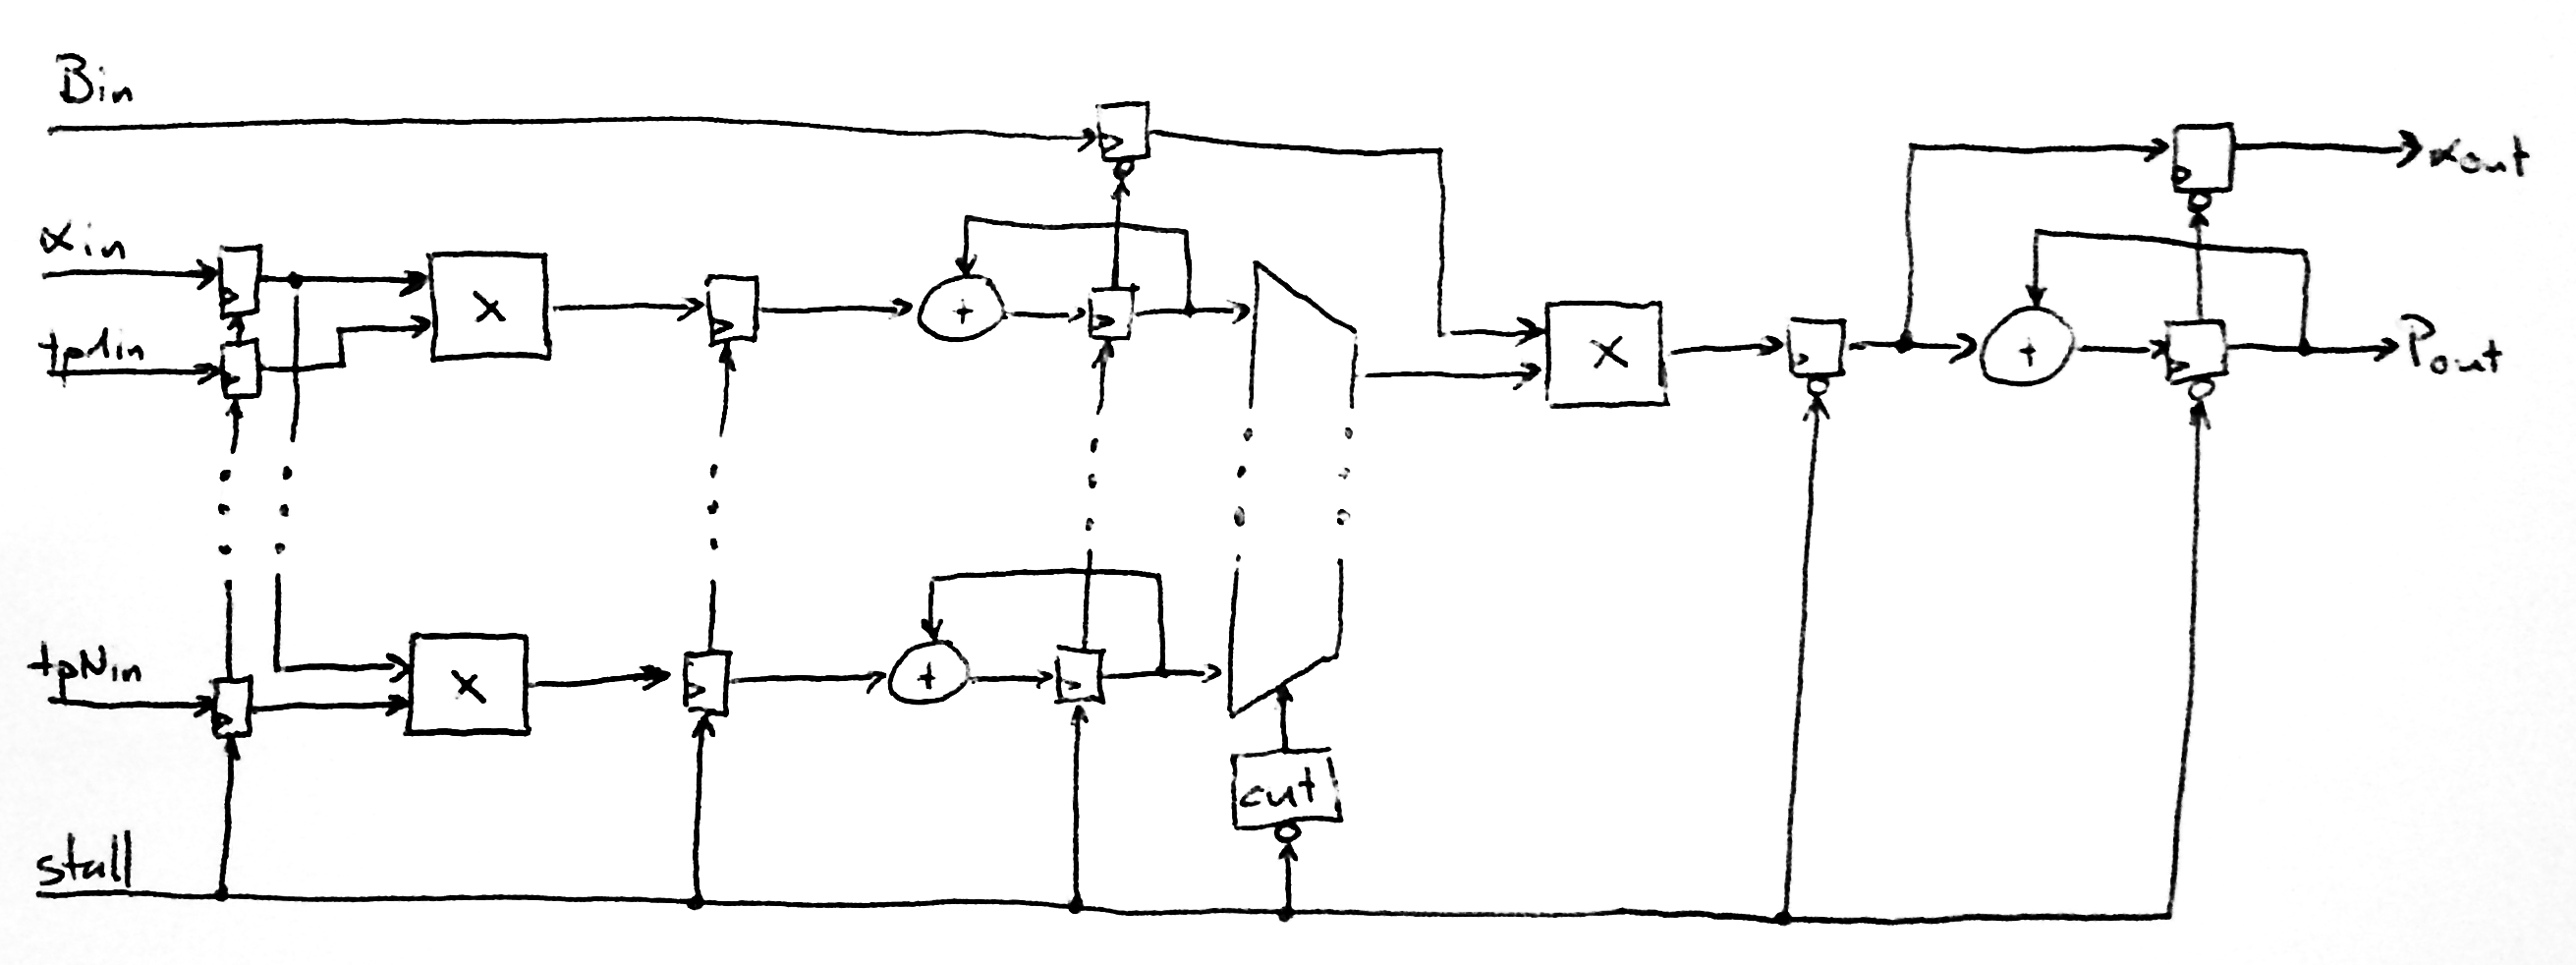
\includegraphics[width=1\columnwidth]{arch_step_p.png}
    \caption{k-th step with $ N+1 $ MACC units and integrated computation of P
        (which is only needed at the last step)}
    \label{fig:step_p}
\end{figure}

%-------------------------------------------------------------------------------
\subsection{Serial Controller}

\begin{figure}[h]
    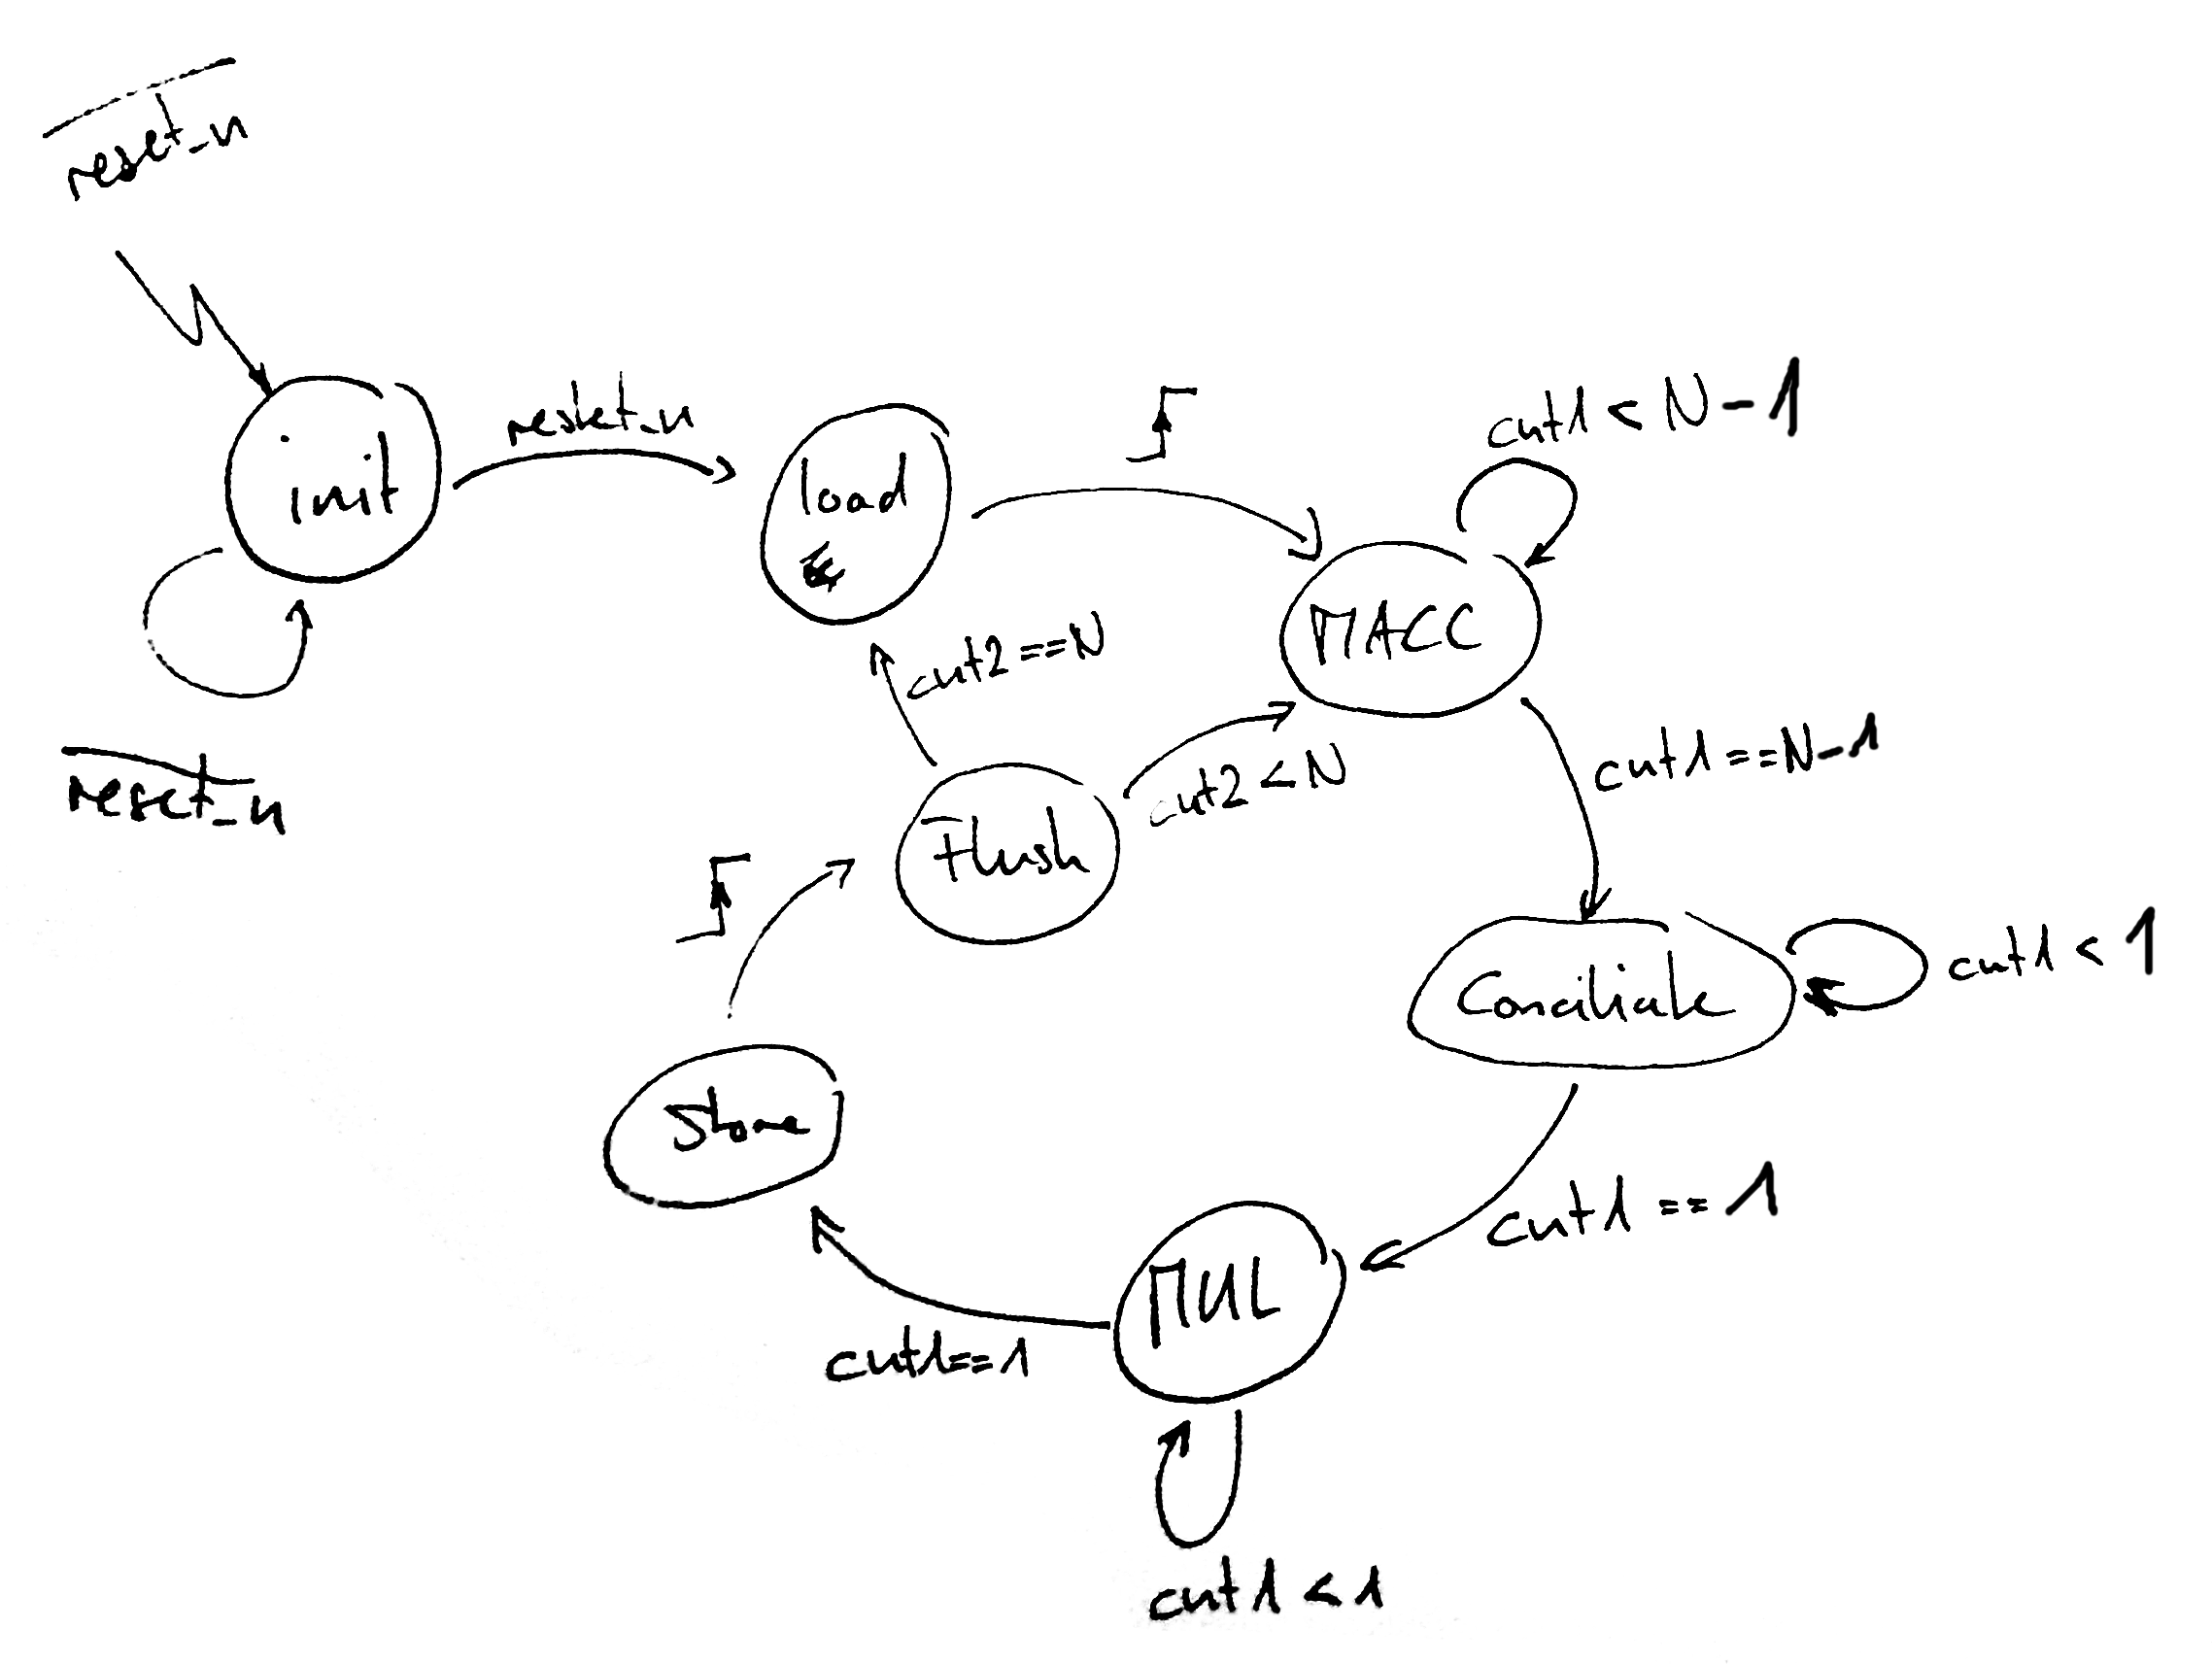
\includegraphics[width=1\columnwidth]{arch_ctrl.png}
    \caption{Controller of serial implementation}
    \label{fig:ctrl}
\end{figure}

\begin{table}[H]
    \label{tab:ctrl}
    \begin{center}
    \begin{tabular}{|l|c|c|c|c|c|c|c|}
    \hline
                      & INIT & LOAD & MACC & CONCILIATE & MUL & STORE & FLUSH \\
    \hline
    sel\_op1          & 0    & 0    & 0    & 0          & 1   & 0     & 0     \\
    sel\_op1\_zero    & 0    & 0    & 0    & 1          & 0   & 0     & 0     \\
    sel\_op2          & 0    & 0    & 0    & 0          & 1   & 0     & 0     \\
    load\_alpha\_in   & 0    & 1    & 0    & 0          & 0   & 0     & 0     \\
    load\_out         & 0    & 0    & 0    & 0          & 0   & 1     & 0     \\
    shift\_alpha\_in  & 0    & 1    & 1    & 0          & 0   & 0     & 0     \\
    shift\_alpha\_out & 0    & 0    & 0    & 0          & 0   & 1     & 0     \\
    enable\_init      & 0    & 0    & 0    & 0          & 1   & 0     & 0     \\
    enable\_step      & 0    & 0    & 1    & 1          & 1   & 0     & 0     \\
    enable\_final     & 0    & 0    & 1    & 0          & 0   & 0     & 0     \\
    flush             & 0    & 0    & 0    & 0          & 0   & 0     & 1     \\
    flush\_Ps         & 0    & 1    & 0    & 0          & 0   & 0     & 0     \\
    \hline
    \end{tabular}
    \end{center}
    \caption{Control signals}
\end{table}

%-------------------------------------------------------------------------------
\subsection{Balancing Pipeline Stages}

%===============================================================================
%%%%%%%%%%%%%%%%%%%%%%%%%%%%%%%%%%%%%%%%%%%%%%%%%%%%%%%%%%%%%%%%%%%%%%%%%%%%%%%%
\chapter{Testing and Verification}
\label{ch:test}

%-------------------------------------------------------------------------------
%===============================================================================
\section{Device}
\label{ch:test_dev}

\begin{itemize}
    \item Nexys4 board with Artix-7 FPGA
    \item limited recourses -> proof of concept
    \item bord hardware for testing
\end{itemize}

%-------------------------------------------------------------------------------
%===============================================================================
\section{Relation to Proposed Algorithm}
\label{ch:test_prop}

%-------------------------------------------------------------------------------
\subsection{Log Standard}

%-------------------------------------------------------------------------------
\subsection{Metrics}

%===============================================================================
%%%%%%%%%%%%%%%%%%%%%%%%%%%%%%%%%%%%%%%%%%%%%%%%%%%%%%%%%%%%%%%%%%%%%%%%%%%%%%%%
\chapter{Results}
\label{ch:res}
%-------------------------------------------------------------------------------
\section{Speedup}
\label{ch:res_speed}
%-------------------------------------------------------------------------------
\section{Accuracy}
\label{ch:res_prec}

%===============================================================================
%%%%%%%%%%%%%%%%%%%%%%%%%%%%%%%%%%%%%%%%%%%%%%%%%%%%%%%%%%%%%%%%%%%%%%%%%%%%%%%%
\chapter{Conclusion}
\label{ch:conc}

%-------------------------------------------------------------------------------
%===============================================================================
\section{Achievements}
\label{ch:conc_ach}

%-------------------------------------------------------------------------------
%===============================================================================
\section{Future Work}
\label{ch:conc_work}

\nocite{*}

\appendix %optional, use only if you have an appendix

%===============================================================================
%%%%%%%%%%%%%%%%%%%%%%%%%%%%%%%%%%%%%%%%%%%%%%%%%%%%%%%%%%%%%%%%%%%%%%%%%%%%%%%%
\chapter{Some material}
%\section{It's over\dots}

\backmatter

%\chapter{Glossary} %optional

%\bibliographystyle{alpha}
%\bibliographystyle{dcu}
%\bibliographystyle{plainnat}
%\bibliographystyle{plain}
%\bibliographystyle{abbrvnat}
\bibliographystyle{siam}
%\bibliographystyle{ieeetr}
\bibliography{biblio}

%\cleardoublepage
%\theindex %optional, use only if you have an index, must use
	  %\makeindex in the preamble

\end{document}
